% Copyright 2004 by Till Tantau <tantau@users.sourceforge.net>.
%
% In principle, this file can be redistributed and/or modified under
% the terms of the GNU Public License, version 2.
%
% However, this file is supposed to be a template to be modified
% for your own needs. For this reason, if you use this file as a
% template and not specifically distribute it as part of a another
% package/program, I grant the extra permission to freely copy and
% modify this file as you see fit and even to delete this copyright
% notice. 

\documentclass{beamer}
% Replace the \documentclass declaration above
% with the following two lines to typeset your 
% lecture notes as a handout:
%\documentclass{article}
\usepackage{CJKutf8}
\usepackage[T1]{fontenc}
%\usepackage[utf8x]{inputenc}
\usepackage{graphicx}


% There are many different themes available for Beamer. A comprehensive
% list with examples is given here:
% http://deic.uab.es/~iblanes/beamer_gallery/index_by_theme.html
% You can uncomment the themes below if you would like to use a different
% one:
%\usetheme{AnnArbor}
%\usetheme{Antibes}
%\usetheme{Bergen}
%\usetheme{Berkeley}
%\usetheme{Berlin}
%\usetheme{Boadilla}
%\usetheme{boxes}
%\usetheme{CambridgeUS}
%\usetheme{Copenhagen}
%\usetheme{Darmstadt}
%\usetheme{default}
%\usetheme{Frankfurt}
\usetheme{Goettingen}
%\usetheme{Hannover}
%\usetheme{Ilmenau}
%\usetheme{JuanLesPins}
%\usetheme{Luebeck}
%\usetheme{Madrid}
%\usetheme{Malmoe}
%\usetheme{Marburg}
%\usetheme{Montpellier}
%\usetheme{PaloAlto}
%\usetheme{Pittsburgh}
%\usetheme{Rochester}
%\usetheme{Singapore}
%\usetheme{Szeged}
%\usetheme{Warsaw}

\begin{document}
\begin{CJK}{UTF8}{gbsn}

\title{竞价排名系统-VPAS}

% A subtitle is optional and this may be deleted
\subtitle{功能简介、结构设计与接入标准}

\author{李庚\inst{1}}
% - Give the names in the same order as the appear in the paper.
% - Use the \inst{?} command only if the authors have different
%   affiliation.

\institute[Qunar.com] % (optional, but mostly needed)
{
  \inst{1}%
  旅游度假SI \\
  新业务部
}
% - Use the \inst command only if there are several affiliations.
% - Keep it simple, no one is interested in your street address.

\date{Jan. 20th, 2013}
% - Either use conference name or its abbreviation.
% - Not really informative to the audience, more for people (including
%   yourself) who are reading the slides online

\subject{2014技术分享}
% This is only inserted into the PDF information catalog. Can be left
% out. 

% If you have a file called "university-logo-filename.xxx", where xxx
% is a graphic format that can be processed by latex or pdflatex,
% resp., then you can add a logo as follows:

% \pgfdeclareimage[height=0.5cm]{university-logo}{university-logo-filename}
% \logo{\pgfuseimage{university-logo}}

% Delete this, if you do not want the table of contents to pop up at
% the beginning of each subsection:
\AtBeginSubsection[]
{
  \begin{frame}<beamer>{纲要}
    \tableofcontents[currentsection,currentsubsection]
  \end{frame}
}

% Let's get started

\begin{frame}
  \titlepage
\end{frame}

\begin{frame}{纲要}
  \tableofcontents
  % You might wish to add the option [pausesections]
\end{frame}

% Section and subsections will appear in the presentation overview
% and table of contents.
\section{功能介绍}

\begin{frame}{系统目标}
  \begin{itemize}
  \item {
    为产品供应商提供通过产品点击单价获取展示的功能,允许供应商通过提高产品点击单价的方式获取更好的展示排名
  }
  \end{itemize}
\end{frame}

\begin{frame}{应用举例}
  \begin{block}{度假搜索列表页}
    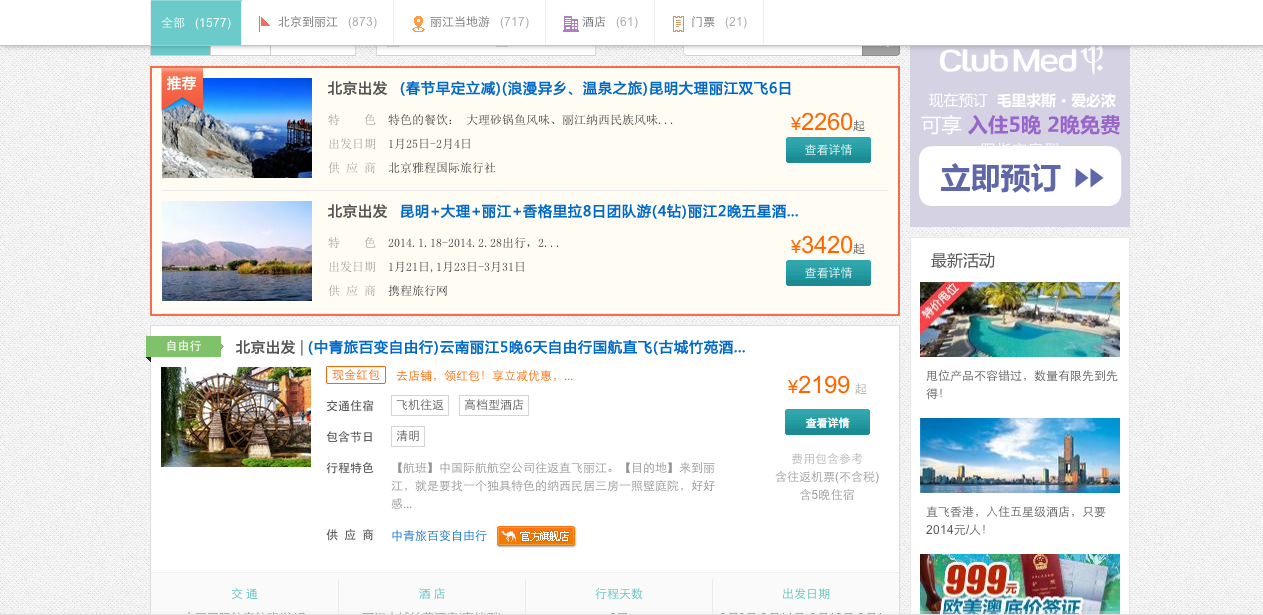
\includegraphics[scale=0.22]{./imgs/overview-qunar}
  \end{block}
\end{frame}

\begin{frame}{应用举例}
  \begin{block}{百度知心卡片}
    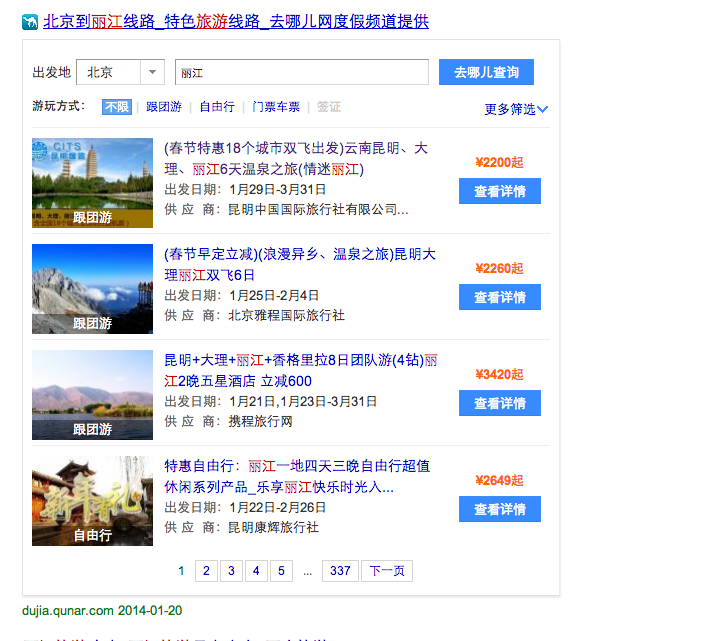
\includegraphics[scale=0.3]{./imgs/overview-baidu}
  \end{block}
\end{frame}

\subsection{竞价产品投放}
\begin{frame}{竞价产品投放}
  \begin{itemize}
  \item {
    精确设置产品竞价的时间计划
    \pause
  }
  \item {
    日消费限额计划
  }
  \end{itemize}
\end{frame}


\subsection{竞价展示排序}

\begin{frame}{竞价展示排序}
  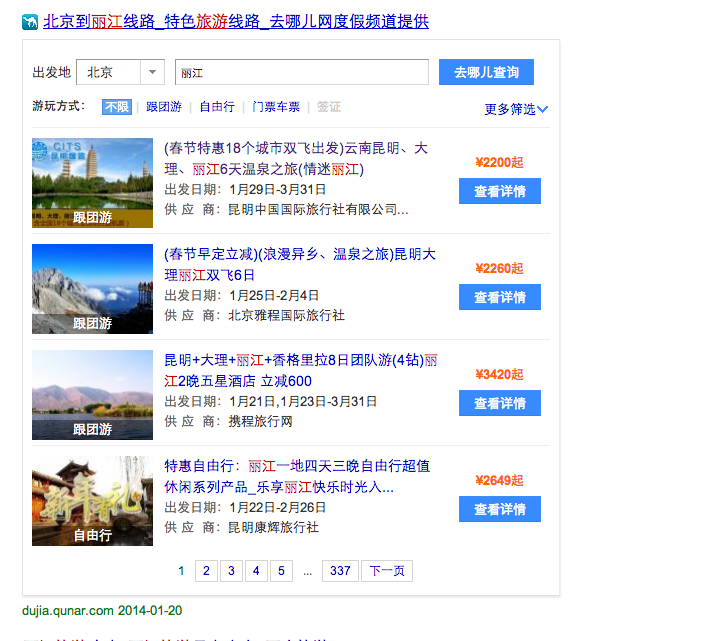
\includegraphics[scale=0.25]{./imgs/overview-baidu}
  \begin{itemize}
  \item {
    精确匹配产品的竞价关键词
    \pause
  }
  \item {
    综合产品质量以及点击单价计算排名
  }
  \end{itemize}
\end{frame}

\subsection{点击计费结算}

\begin{frame}{点击计费结算}
  \begin{itemize}
  \item {
    实时点击扣费
  }
  \item {
    无效点击识别,实时返款
  }
  \item {
    综合全天的点击情况,产生日结算报表,平账
  }
  \end{itemize}
\end{frame}

% \subsection{Second Subsection}

% You can reveal the parts of a slide one at a time
% with the \pause command:
%% \begin{frame}{Second Slide Title}
%%   \begin{itemize}
%%   \item {
%%     First item.
%%     \pause % The slide will pause after showing the first item
%%   }
%%   \item {   
%%     Second item.
%%   }
%%   % You can also specify when the content should appear
%%   % by using <n->:
%%   \item<3-> {
%%     Third item.
%%   }
%%   \item<4-> {
%%     Fourth item.
%%   }
%%   % or you can use the \uncover command to reveal general
%%   % content (not just \items):
%%   \item<5-> {
%%     Fifth item. \uncover<6->{Extra text in the fifth item.}
%%   }
%%   \end{itemize}
%% \end{frame}

\section{结构设计}

\subsection{技术基础}

\begin{frame}{技术基础}
\begin{block}{QADS文字链广告系统}
  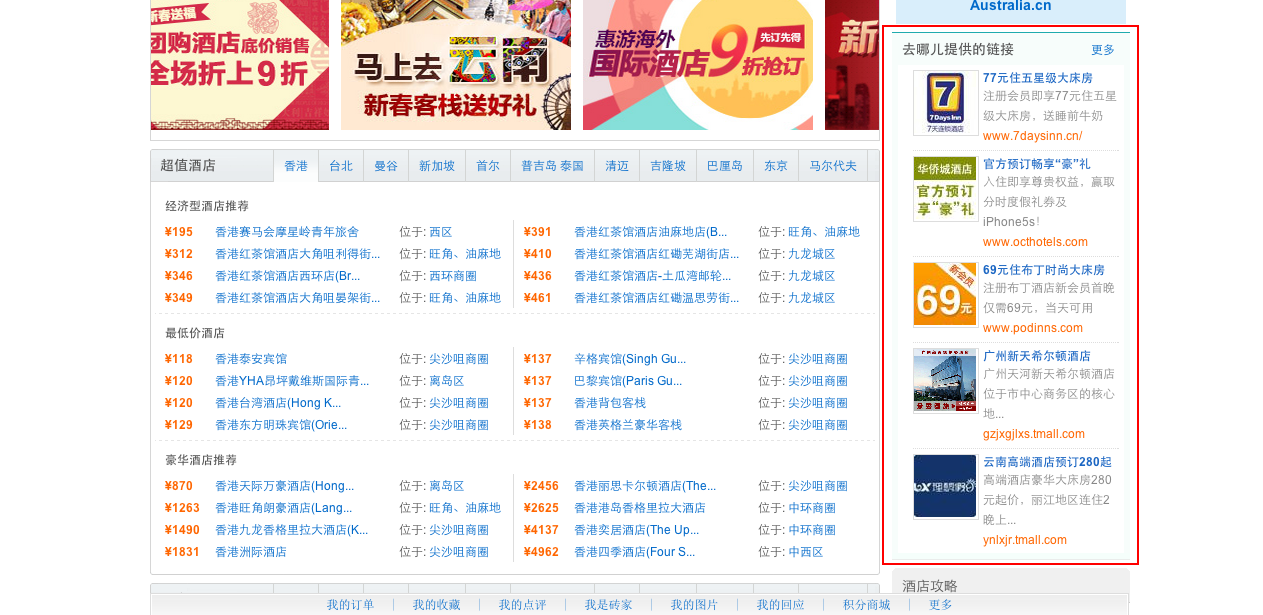
\includegraphics[scale=0.23]{./imgs/qads-demo}
  \pause
\end{block}
\begin{block}{稳定的功能:主要的产品线上都有应用}
  \begin{itemize}
    \item {
      竞价展示排序 
    }
    \item {
      点击计费结算 
    }
  \end{itemize}
\end{block}
\end{frame}

\subsection{难点与挑战}

\begin{frame}{难点与挑战}
  \begin{block}{功能整合}
    \begin{itemize}
      \item {
        原本的度假业务系统在初始设计上无竞价的考虑
      }
      \item {
        原本的QADS文字链广告系统在设计上与业务产品无关
      }
    \end{itemize}
    \pause
  \end{block}
  \begin{block}{需求和技术的矛盾}
    \begin{itemize}
    \item {
      需求:希望尽快看到度假产品竞价接入的结果和效果
    }
    \item {
      技术:实现通用的竞价接入框架,避免过度耦合
    }
    \end{itemize}
    \pause
  \end{block}
  \begin{block}{项目总开发时间较短}
    \begin{itemize}
      \item {
        设计上出错补救的机会几乎没有
      }
      \item {
        较难处理一开始不够清晰的产品需求
      }
    \end{itemize}
  \end{block}
\end{frame}

\subsection{系统设计原则}

\begin{frame}{系统设计原则}
  \begin{block}{严格定义系统边界}
    业务属性与竞价产品属性严格分离,产品竞价系统不能处理业务相关的逻辑
  \end{block}
  \begin{block}{避免对功能稳定的部分做修改或者重新开发}
    \begin{itemize}
      \item {
        关键模块逻辑复杂,且容易产生灾难性的结果。例如:扣费结算
      }
      \item {
        回归测试代价高,容易拖慢整体上线进度
      }
    \end{itemize}
  \end{block}
\end{frame}

\section{产品接入标准} 

% Placing a * after \section means it will not show in the
% outline or table of contents.
\section*{Summary}

\begin{frame}{Summary}
  \begin{itemize}
  \item
    The \alert{first main message} of your talk in one or two lines.
  \item
    The \alert{second main message} of your talk in one or two lines.
  \item
    Perhaps a \alert{third message}, but not more than that.
  \end{itemize}
  
  \begin{itemize}
  \item
    Outlook
    \begin{itemize}
    \item
      Something you haven't solved.
    \item
      Something else you haven't solved.
    \end{itemize}
  \end{itemize}
\end{frame}



% All of the following is optional and typically not needed. 
\appendix
\section<presentation>*{\appendixname}
\subsection<presentation>*{For Further Reading}

\begin{frame}[allowframebreaks]
  \frametitle<presentation>{For Further Reading}
    
  \begin{thebibliography}{10}
    
  \beamertemplatebookbibitems
  % Start with overview books.

  \bibitem{Author1990}
    A.~Author.
    \newblock {\em Handbook of Everything}.
    \newblock Some Press, 1990.
 
    
  \beamertemplatearticlebibitems
  % Followed by interesting articles. Keep the list short. 

  \bibitem{Someone2000}
    S.~Someone.
    \newblock On this and that.
    \newblock {\em Journal of This and That}, 2(1):50--100,
    2000.
  \end{thebibliography}
\end{frame}

\clearpage
\end{CJK}
\end{document}
